\title{Лекция 4\\Внешние языки представления информации}   
\author[]{Шункевич Д.В.}
\institute[]{Белорусский государственный университет информатики и радиоэлектроники}

\begin{frame}
	\titlepage
\end{frame}

\begin{frame}{\\Содержание лекции}
	\topline
	\justifying
	Графический язык внешнего представления конструкций SC-кода – SCg-код. Синтаксис и денотационная семантика SCg-кода. Линейный язык внешнего представления конструкций SC-кода – SCs-код. Синтаксис и денотационная семантика SCs-кода. Структурированный гипертекстовый язык внешнего представления конструкций SC-кода – SCn-код.
\end{frame}

\begin{frame}{\\Понятие внешних языков}
	\topline
	\justifying
	\begin{SCn}
		\scnheader{внешний язык}
		\scnidtf{язык представление информации, которую видит и понимает человек}
		\scnidtf{язык обмена сообщениями}
		\begin{scnrelfromset}
			{\textit{примеры}}
			\scnitem {SCn-код}
			\scnitem {SCs-код}
			\scnitem {SCg-код}
		\end{scnrelfromset}
		\scnheader{внутренний язык}
		\scnidtf{язык представления информации в памяти кибернетической системы}
	\end{SCn}

\end{frame}

\begin{frame}{\\SCg-код}
	\topline
	\justifying
	\vspace*{\fill}
	\begin{SCn}
		\scnheader{SCg-код}
		\scnidtf{Semantic Code graphical}
		\scnidtf{Язык визуального (графического) представления баз знаний ostis-систем}
		\scniselement{графовый язык}
		\scntext{пояснение}{\textit{SCg-код} представляет собой способ визуализации \textit{sc-текстов} (информационных конструкций SC-кода) в виде рисунков этих абстрактных конструкций. Подчеркнем, что абстрактная \textit{графовая структура} и её рисунок (графическое изображение) – это не одно и то же даже если они изоморфны друг другу. \textit{SCg-код} рассматривается нами как объединение \textit{Ядра SCg-кода}, обеспечивающего изоморфное графическое изображение любого \textit{sc-текста}, а также нескольких направлений расширения этого ядра, обеспечивающих повышение компактности и "читабельности" текстов \textit{SCg-кода (sc.g-текстов).}}
	\end{SCn}
\end{frame}

\begin{frame}{\\SCg-код}
	\topline
	\justifying
	\vspace*{\fill}\\
	Основная цель \textit{SCg-кода} – иметь четкие синтаксические графические признаки изображения \textit{sc.g-элементов}, позволяющие легко выделить и различать такие классы \textit{sc.g-элементов}, как:
	\begin{textitemize}
		\item \textit{ sc.g-константы} (знаки константных сущностей) и \textit{sc.g-переменные} (изображения переменных, значениями которых являются соответствующие sc-элементы);
		\item \textit{sc.g-переменные}, значениями которых являются {sc-константы}, и \textit{sc.g-переменные}, значениями которых являются \textit{sc-переменные};
		\item знаки постоянных (стабильных) сущностей и знаки временных (нестабильных, временно существующих, ситуативных) сущностей;
	\end{textitemize}
	
\end{frame}

\begin{frame}{\\SCg-код}
	\topline
	\justifying
	\begin{textitemize}
		\item \textit{sc.g-коннекторы} (знаки бинарных связей) и \textit{sc.g-элементы}, не являющиеся \textit{sc.g-коннекторами};
		\item неориентированные \textit{sc.g-коннекторы (sc.g-ребра)} и ориентированные \textit{(sc.g-дуги)};
		\item \textit{sc.g-дуги принадлежности} и \textit{sc.g-дуги}, не являющиеся таковыми;
		\item \textit{sc.g-дуги позитивной принадлежности}, негативной принадлежности и нечеткой принадлежности.
	\end{textitemize}
\end{frame}

\begin{frame}{\\Синтаксис SCg-кода}
	\topline
	\justifying
	\begin{SCn}
		\scnheader{Алфавит Ядра SCg-кода}
		\scnidtf{Алфавит sc.g-элементов, графически изображающих sc-элементы}
	\end{SCn}
	В таблице \textbf{“SCg-текст. Алфавит SCg-кода”} приведен перечень элементов \textbf{Алфавита SCg-кода}. Этот перечень оформлен в виде \textit{sc.g-текста} и представляет собой изображение примеров всех введенных видов \textit{sc.g-элементов} (по одному примеру каждого вида). При этом, указанные примеры \textit{sc.g-элементов} разбиты на пять групп.
\end{frame}
\begin{frame}{\\Синтаксис SCg-кода}
	\topline
	\justifying
	\vspace*{\fill}
	\begin{figure}[H]
		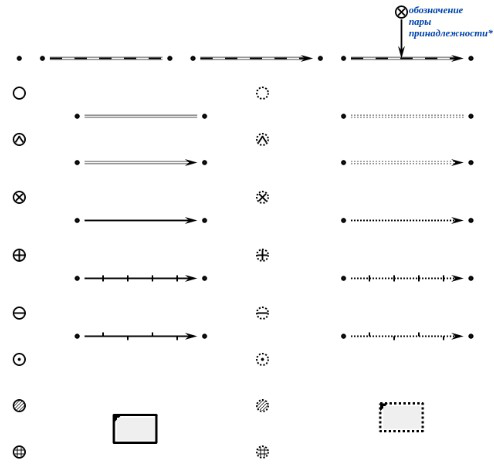
\includegraphics[scale=0.55]{./figures/external_langs/alphabet_scg_code_part1.png}
	\end{figure}
\end{frame}

\begin{frame}{\\Синтаксис SCg-кода}
	\topline
		\justifying
	\vspace*{\fill}
	\begin{figure}[H]
		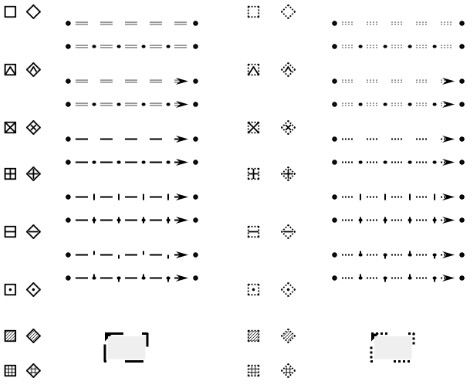
\includegraphics[scale=0.6]{./figures/external_langs/alphabet_scg_code_part2.png}
	\end{figure}
\end{frame}

\begin{frame}{\\Синтаксис SCg-кода}
	\topline
	\justifying
	\vspace*{\fill}\\
	\small{Первая группа (верхняя строка) включает в себя \textit{sc.g-элементы}, для которых кон стантность и постоянство обозначаемых ими сущностей требует дополнительного уточнения. Остальные четыре группы \textit{sc.g-элементов} аналогичны друг другу и включают в себя соответственно:
	\begin{textitemize}
		\item знаки \textbf{константных постоянных сущностей};
		\item знаки \textbf{константных временных сущностей};
		\item изображения \textit{sc-переменных}, значениями которых или значениями значений которых (в случае, если значениями переменных являются переменные) являются знаки константных постоянных сущностей;
		\item изображения \textit{sc-переменных}, значениями которых или значениями значений которых (в случае, если значениями переменных являются переменные) являются знаки константных временных сущностей.
	\end{textitemize}}
\end{frame}

\begin{frame}{\\Синтаксис SCg-кода}
	\topline
	\justifying
	Особое место в SCg-коде занимает изображение \textit{sc-элементов}, являющихся \textit{обозначениями пар принадлежности*}, путём явного использования этого \textit{\underline{семантически} выделяемого класса sc-элементов}. Данный \textit{sc.g-элемент} используется тогда, когда нам необходимо изобразить \textit{sc-дугу}, о которой известно, что она является обозначением \textit{пары принадлежности*}, но неизвестно о какой принадлежности идет речь – о константной или переменной, о
	постоянной или временной, о позитивной, негативной или нечеткой.
\end{frame}

\begin{frame}{\\Синтаксис SCg-кода}
	\topline
	\justifying
	\vspace*{\fill}\\
	Кроме \textit{sc.g-элементов}, перечисленных в таблице \textbf{“SCg-текст. Алфавит SCg-кода”}, в состав \textit{Алфавита SCg-кода} входят также следующие \textit{sc.g-элементы}:
	\begin{textitemize}
		\item внешние идентификаторы \textit{sc-элементов}, идентичные (приписываемые) соответствующим \textit{sc.g-элементам};
		\item \textit{sc.g-контура}, каждый из которых является знаком некоторого \textit{sc-текста} (структуры, состоящей из sc-элементов);
		\item \textit{sc.g-рамки} увеличенного размера являются ограничителями изображения различных файлов, хранимых в памяти ostis-системы;
		\item \textit{sc.g-шины}, являющиеся обозначениями тех же сущностей, что и инцидентные им \textit{sc.g-элементы}.
	\end{textitemize}
\end{frame}

\begin{frame}{\\Синтаксис SCg-кода}
	\topline
	\justifying
	\vspace*{\fill}\\
	Заметим также, что, кроме всех перечисленных элементов \textit{Алфавита SCg-кода}, каждый из которых имеет вполне определенную денотационную семантику, для формализации синтаксиса SCg-кода необходимо ввести целый ряд более "мелких" синтаксических объектов, например:
	\begin{textitemize}
		\item точек инцидентности \textit{sc.g-коннекторов} с \textit{sc.g-узлами}, с другими \textit{sc.g-коннекторами, с sc.g-контурами, с sc.g-рамками};
		\item точек инцидентности \textit{sc.g-шин};
		\item точек излома линейных \textit{sc.g-элементов (sc.g-коннекторов, sc.g-контуров, sc.g-рамок, sc.g-шин)}.
	\end{textitemize}
\end{frame}

\begin{frame}{\\Денотационная семантика SCg-кода}
	\topline
	\justifying
	\vspace*{\fill}\\
	В SCg-коде выделяются \textit{Ядро SCg-кода} и его расширения. \textit{Алфавит Ядра SCg-кода} – алфавит \textit{sc.g-элементов}, графически изображаемых \textit{sc-элементы}. \textit{Алфавит Ядра SCg-кода} взаимно однозначно соответствует \textit{Алфавиту SC-кода}.
	Денотационная семантика \textit{Ядра SCg-кода} соответствует денотационной семантике SC-кода.
	\begin{figure}[H]
		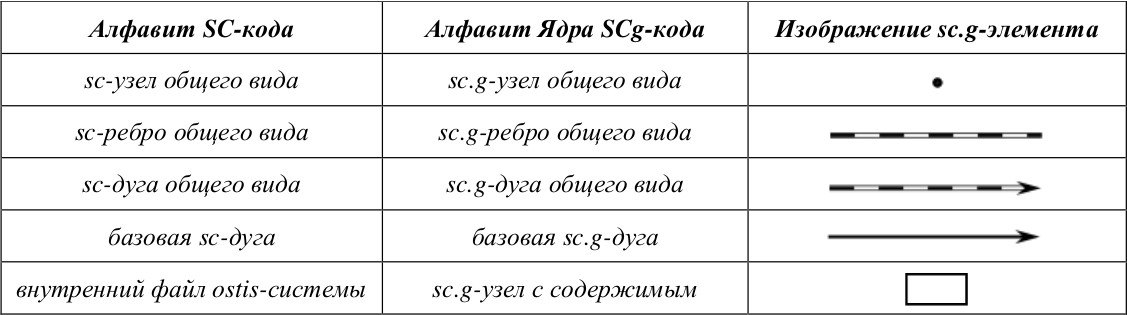
\includegraphics[scale=0.4]{./figures/external_langs/table_scg_code.png}
	\end{figure}
\end{frame}

\begin{frame}{\\Денотационная семантика SCg-кода}
	\topline
	\justifying
	\begin{SCn}
		\scnheader{sc.g-узел общего вида}
		\scnidtf{\textit{sc.g-элемент}, являющийся графическим изображением \textit{sc-узла общего вида}}
		\scntext{\textit{пояснение}}{Все \textit{sc-узлы}, не являющиеся знаками файлов, в тексте (конструкции) \textit{Ядра SCg-кода}, изображаются в виде небольших чёрных кругов одинакового диаметра, который обозначим через \textbf{d}, и точная величина которого зависит от масштаба отображения \textit{sc.g-текста}.}
		
	\end{SCn}
\end{frame}

\begin{frame}{\\Денотационная семантика SCg-кода}
	\topline
	\justifying
	\begin{SCn}
		\scnheader{sc.g-ребро общего вида}
		\scnidtf{\textit{sc.g-элемент}, являющийся графическим изображением \textit{sc-ребра общего вида}}
		\scntext{\textit{пояснение}}{Каждое \textit{sc-ребро} в \textit{Ядре SCg-кода} изображается в виде широкой линии, в которой чередуются фрагменты со сплошной заливкой и без заливки, не имеющей самопересечений и имеющей общую толщину, равную примерно \textbf{0.7d}.}
	\end{SCn}
\end{frame}

\begin{frame}{\\Денотационная семантика SCg-кода}
	\topline
	\justifying
	\begin{SCn}
		\scnheader{sc.g-дуга общего вида}
		\scnidtf{\textit{sc.g-элемент}, являющийся графическим изображением \textit{sc-дуги общего вида}}
		\scntext{\textit{пояснение}}{Каждая \textit{sc-дуга} в \textit{Ядре SCg-кода} изображается в виде широкой линии, в которой чередуются фрагменты со сплошной заливкой и без заливки, не имеющей самопересечений и имеющей общую толщину, равную примерно \textbf{0.7d} и имеющей изображение стрелочки на одном из концов этой линии.}
	\end{SCn}
\end{frame}

\begin{frame}{\\Денотационная семантика SCg-кода}
	\topline
	\justifying
	\begin{SCn}
		\scnheader{базовая sc.g-дуга}
		\scnidtf{\textit{sc.g-элемент}, являющийся графическим изображением \textit{базовой sc-дуги}}
		\scntext{\textit{пояснение}}{Каждая входящая в состав \textit{sc-текста} базовая \textit{sc-дуга} в \textit{Ядре SCg-кода} изображается в виде линии произвольной формы, не имеющий самопересечений, имеющий толщину \textbf{0.4d} , и имеющей изображение стрелочки на одном из ее концов.}
	\end{SCn}
\end{frame}

\begin{frame}{\\Денотационная семантика SCg-кода}
	\topline
	\justifying
	\begin{SCn}
		\scnheader{внутренний файл ostis-системы}
		\scnidtf{\textit{sc-узел}, являющийся знаком внутреннего файла ostis-системы}
		\scnidtf{\textit{sc-узел} с содержимым}
		\scnidtf{\textit{sc-знак} внутреннего файла ostis-системы}
	\end{SCn}
\end{frame}

\begin{frame}{\\Денотационная семантика SCg-кода}
	\topline
	\justifying
	\begin{SCn}
		\scnheader{\textit{sc-узел} с содержимым}
		\scnidtf{\textit{sc-узел}, имеющий содержимое}
		\scnidtf{\textit{sc-узел}, являющийся знаком внутреннего файла ostis-системы}
		\scnidtf{\textit{sc-знак} внутреннего файла ostis-системы}
		\scnidtf{\textit{sc.g-рамка}, ограничивающая изображение (представление) внутреннего файла ostis-системы, обозначаемого этой \textit{sc.g-рамкой}}
		\scntext{\textit{пояснение}}{Каждый входящий в sc-текст \textit{sc-узел}, имеющий содержимое, в \textit{Ядре SCg-кода} изображается в виде прямоугольника произвольного размера с толщиной линии \textbf{0.6d}. Внутри этого прямоугольника отображается \textit{файл}, обозначаемый изображаемым \textit{sc-узлом}. Если нет необходимости изображать в тексте сам файл, то \textit{sc-узел}, обозначающий такой \textit{файл}, в \textit{sc.g-тексте} изображается в виде прямоугольника со сторонами \textbf{2d} по вертикали и \textbf{4d} по горизонтали.}
	\end{SCn}
\end{frame}

\begin{frame}{\\SCs-код}
	\topline
	\justifying
	\vspace*{\fill}\\
		\begin{SCn}
			\scnheader{SCs-код}
			\scnidtf{Semantic Code string}
			\scnidtf{Язык линейного представления знаний ostis-систем}
			\scnidtf{Множество всевозможных текстов SCs-кода}
			\scnidtf{Язык внешнего линейного представления конструкций внутреннего языка ostis-систем}
			\scntext{\textit{пояснение}}{SCs-код представляет собой множество линейных текстов \textit{(sc.s- текстов)}, каждый из которых состоит из предложений \textit{(sc.s-предложений)}, разделенных друг от друга \textit{двойной точкой с запятой} (разделителем \textit{sc.s-предложений}). При этом \textit{sc.s-предложение} представляет собой последовательность \textit{sc-идентификаторов}, являющихся именами описываемых сущностей и разделяемых между собой различными \textit{sc.s-разделителями} и \textit{sc.s-ограничителями}.}
		\end{SCn}
\end{frame}

\begin{frame}{\\Синтаксис SCs-кода}
	\topline
	\justifying
	\vspace*{\fill}\\
	\small{
		\begin{SCn}
			\scnheader{Алфавит SCs-кода}
			\scnidtf{Алфавит символов SCs-кода}
			\scnidtf{множество символов SCs-кода}
			\scnidtf{символ, используемый в текстах SCs-кода}
			\scnidtf{Язык внешнего линейного представления конструкций внутреннего языка ostis-систем}
			\scntext{\textit{пояснение}}{\textit{Алфавит SCs-кода} строится на основе современных общепринятых наборов символов, что позволяет упростить разработку средств для работы с \textit{sc.s-текстами} с использованием современных технологий. В состав \textit{sc.s-текстов}, как и в состав текстов любых других языков, являющихся вариантами внешнего отображения текстов SC-кода, могут входить различные файлы, в том числе естественно-языковые или даже файлы, содержащие другие \textit{sc.s-тексты}. В общем случае в таких файлах могут использоваться самые разные символы, в связи с чем будем считать, что в \textit{Алфавит SCs-кода} эти символы не включаются.}
		\end{SCn}
	}
\end{frame}

\begin{frame}{\\Синтаксис SCs-кода}
	\topline
	\justifying
	\vspace*{\fill}\\
	\small{
		\begin{SCn}
			\scnheader{Алфавит символов, используемых в sc.s-разделителях}
			\scnhaselement{\textit{пробел}; \textit{точка с запятой}; \textit{двоеточие}; \textit{круглый маркер}; \textit{знак равенства}}
			\scnsuperset{Алфавит символов, используемых в sc.s-разделителях, изображающих связь инцидентности sc-элементов}
			\begin{scnindent}
				\scnhaselement{![ > ]!; ![ < ]!; ![ | ]!; ![ - ]!;}
			\end{scnindent}
			\scnsuperset{Алфавит символов, используемых в sc.s-коннекторах}
			\begin{scnindent}
				\scnsuperset{Расширенный алфавит символов, используемых в sc.s-коннекторах}
				\begin{scnindent}
					\scnidtf{Расширенный алфавит sc.s-коннекторов}
					\scnhaselement{![$\in$]!; ![$\ni$]!; ![$\notin$]!; ![$\not\ni$]!; ![$\subseteq$]!; ![$\supseteq$]!; ![$\subset$]!; ![$\supset$]!; ![$\leq$]!; ![$\geq$]!; ![$\Leftarrow$]!; ![$\Rightarrow$]!; ![$\Leftrightarrow$]!; ![$\leftarrow$]!; ![$\rightarrow$]!; ![$\leftrightarrow$]!}
				\end{scnindent}
				\scnsuperset{Базовый алфавит символов, используемых в sc.s-коннекторах}
				\begin{scnindent}
					\scnidtf{Базовый алфавит sc.s-коннекторов}
					\scnhaselement{![$\sim$]!; ~\textit{знак подчеркивания}; ~\textit{знак равенства}; ![ > ]!; ~![<]!; ~\textit{двоеточие}; ![ - ]!; ![ | ]!; ![ / ]!;}
				\end{scnindent}
			\end{scnindent}
		\end{SCn}		
	}
\end{frame}

\begin{frame}{\\Синтаксис SCs-кода}
	\topline
	\justifying
	\vspace*{\fill}\\
	Как в \textit{Базовом}, так и в \textit{Расширенном Алфавитах sc.s-коннекторов} используются следующие общие признаки, характеризующие тип изображаемого \textit{sc-коннектора}:
	\begin{textitemize}
		\item знак подчеркивания как признак изображений  переменных \\ \textit{sc-коннекторов} (один знак подчеркивания для \textit{sc-коннекторов}, являющихся первичными \textit{sc-переменными}, два знака подчеркивания для \textit{sc-коннекторов}, являющихся вторичными \textit{sc-переменными (sc-метапеременными))};
		\item вертикальная черта “ | ” как признак изображений \textit{негативных sc-дуг принадлежности};
		\item косая черта “ / ” как признак изображений \textit{нечетких sc-дуг принадлежности};
		\item тильда “ $\sim$ ” как признак изображений \textit{временных sc-дуг принадлежности}.
	\end{textitemize}
\end{frame}

\begin{frame}{\\Синтаксис SCs-кода}
	\topline
	\justifying
	\vspace*{\fill}\\
	Для упрощения процесса разработки исходных текстов баз знаний с использованием SCs-кода и создания соответствующих средств вводятся два алфавита символов. Базовый алфавит символов, используемых в \textit{sc.s-коннекторах} включает только символы, входящие в переносимый набор символов и имеющиеся на стандартной современной клавиатуре. Таким образом, для разработки исходных текстов баз знаний, использующих только \textit{Базовый алфавит} символов, используемых в \textit{sc.s-коннекторах} достаточно обычного текстового редактора. Расширенный алфавит символов, используемых в \textit{sc.s-коннекторах} включает также дополнительные символы, которые позволяют сделать \textit{sc.s-тексты (и sc.n-тексты)} более читабельными и наглядными. Для визуализации и разработки \textit{sc.s-текстов} с использованием расширенного алфавита требуется наличие специализированных средств
\end{frame}

\begin{frame}{\\Синтаксис SCs-кода}
	\topline
	\justifying
	\vspace*{\fill}\\
	\begin{SCn}
		\scnheader{Алфавит символов, используемых в sc.s-ограничителях}
		\scnhaselement{![ ( ]!; ![ ) ]!; ![ * ]!;}
		
		\scnheader{Алфавит символов, используемых в неоднозначных sc.s-изображениях sc-узлов}
		\scnhaselement{![ \{ ]!; ![ \} ]!; ![ ! ]!; ![ - ]!; ![ [ ]!; ![ ] ]!;}
	\end{SCn}
\end{frame}

\begin{frame}{\\Денотационная семантика SCs-кода}
	\topline
	\justifying
	\vspace*{\fill}\\
	\begin{SCn}
		\begin{figure}[H]
			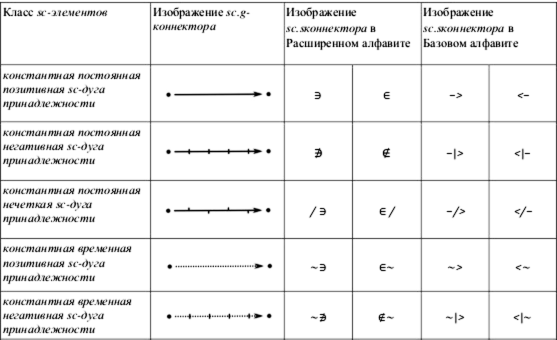
\includegraphics[scale=0.5]{./figures/external_langs/table_scs_1.png}
		\end{figure}
		\end{SCn}
	\end{frame}

\begin{frame}{\\Денотационная семантика SCs-кода}
	\topline
	\justifying
	\vspace*{\fill}\\
	\begin{SCn}
		\begin{figure}[H]
			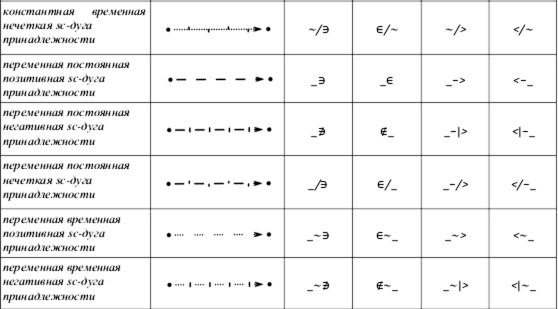
\includegraphics[scale=0.5]{./figures/external_langs/table_scs_2.png}
		\end{figure}
	\end{SCn}
\end{frame}

\begin{frame}{\\Денотационная семантика SCs-кода}
	\topline
	\justifying
	\vspace*{\fill}\\
	\begin{SCn}
		\begin{figure}[H]
			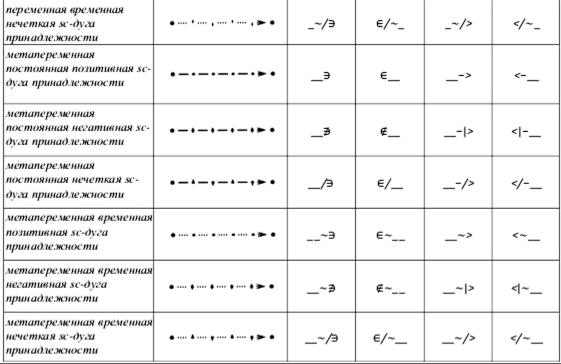
\includegraphics[scale=0.5]{./figures/external_langs/table_scs_3.png}
		\end{figure}
	\end{SCn}
\end{frame}

\begin{frame}{\\SCn-код}
	\topline
	\justifying
	\vspace*{\fill}\\
	\small{
		\begin{SCn}
			\scnheader{SCn-код}
			\scnidtf{Semantic Code natural}
			\scnidtf{Язык структурированного представления знаний ostis-систем}
			\scnidtf{Язык внешнего форматированного представления конструкций внутреннего языка ostis-систем}
			
			\scntext{пояснение}{\textit{SCn-код} является языком структурированного внешнего представления текстов \textit{SC-кода} и представляет собой синтаксическое расширение \textit{SCs-кода}, направленное на повышение наглядности и компактности текстов \textit{SCs-кода}. \textit{SCn-код} позволяет перейти от линейных текстов \textit{SCs-кода} к форматированным и фактически двухмерным текстам, в которых появляется декомпозиция исходного линейного текста \textit{SCs-кода} на строчки, размещенные "по вертикали". При этом начало всех строчек текста фиксировано и определяется известным и ограниченным набором правил, что дает возможность использовать это при форматировании \textit{sc.n-текста} (текста, принадлежащего \textit{SCn-коду}.}
		\end{SCn}
	}
\end{frame}

\begin{frame}{\\SCn-код}
	\topline
	\justifying
	\vspace*{\fill}\\
	Важной особенностью \textit{SCn-кода} является "двухмерный" характер его текстов. Это проявляется в
	том, что для каждого фрагмента текста \textit{SCn-кода} важное значение имеет величина отступа от левого
	края строчки.
	В тексте \textit{SCn-кода} в отличие от текста \textit{SCs-кода} для каждого фрагмента текста важное значение имеет не только то, как этот фрагмент связан с другими фрагментами "по горизонтали"(какой
	фрагмент находится \underline{левее} и какой \underline{правее} на одной и той же \textit{строчке}), но и то, как он связан с другими фрагментами "по вертикали"(какой фрагмент находится \underline{выше} на предыдущей строчке и какой находится \underline{ниже} на следующей строчке). Так, например, если в тексте \textit{SCn-кода} некоторый \textit{sc-идентификатор}(внешний идентификатор \textit{sc-элемента}) размещен сразу после вертикальной табуляционной линии и точно под ним размещен некоторый \textit{sc.s-коннектор}, то это означает, что указанный \textit{sc-элемент} инцидентен \textit{sc-коннектору}, изображенному указанным \textit{sc.s-коннектором}.
\end{frame}

\begin{frame}{\\Синтаксис SCn-кода}
	\topline
	\justifying
	\vspace*{\fill}\\
	Алфавит символов \textit{SCs-кода} является также алфавитом символов и \textit{SCn-кода}, т.е. \textit{алфавиты*} этих языков совпадают.
	\textit{SCn-код} – язык, каждый \textit{текст} которого задается:
	\begin{textitemize}
		\item множеством входящих в него \textit{символов};
		\item отношением порядка (последовательности) \textit{символов} по "горизонтали";
		\item отношением порядка(последовательности) \textit{символов} по "вертикали".
	\end{textitemize}
\end{frame}

\begin{frame}{\\Синтаксис SCn-кода}
	\topline
	\justifying
	\small{
		\begin{SCn}
			\scnheader{sc.n-текст}
			\scnidtf{текст SCn-кода}
			\scnidtf{последовательность предложений SCn-кода}
			\scnidtf{последовательность предложений SCn-кода, каждое из которых не является частью какого-либо другого предложения из \underline{этой} последовательности}
			
			\scnheader{страница sc.n-текста}
			\scnidtf{страница, на которой размещается sc.n-текст}
			
			\scnheader{линия разметки sc.n-текста}
			\scnidtf{табуляционная линия sc.n-текста}
			\scnidtf{вертикальная линия разметки sc.n-текста}
			\scnidtf{вертикальная линия, используемая для упрощения восприятия sc.n-текстов и показывающая уровень отступа для компонентов sc.n-предложений}
		\end{SCn}
	}
\end{frame}

\begin{frame}{\\Синтаксис SCn-кода}
	\topline
	\justifying
	\vspace*{\fill}\\
	\small{
		Все компоненты \textit{sc.s-текстов} используются также и в \textit{sc.n-текстах}:
		\begin{textitemize}
			\item \textit{sc-идентификаторы, sc.s-коннекторы}, модификаторы \textit{sc.s-коннекторов} с соответствующими разделителями (двоеточиями);
			\item разделители, используемые в \textit{sc-выражениях}, обозначающих \textit{sc-множества}, заданные перечислением элементов с соответствующими разделителями (точкой с запятой или круглым маркером);
			\item круглые маркеры в перечислениях идентификаторов \textit{sc-элементов}, связанных однотипными \textit{sc-коннекторами} с однотипными модификаторами с заданным \textit{sc-элементом};
			\item разделители предложений (двойные точки с запятой) (опускаются при преобразовании \textit{sc.s-предложений} в \textit{sc.n-предложения});
			\item ограничители присоединенных \textit{sc.s-предложений} (опускаются при преобразовании \textit{sc.s-предложений} в \textit{sc.n-предложения}).
		\end{textitemize}
	}
\end{frame}

\begin{frame}{\\Синтаксис SCn-кода}
	\topline
	\justifying
	\vspace*{\fill}\\
	В отличие от \textit{sc.s-текстов} в \textit{sc.n-текстах}:
	\begin{textitemize}
		\item добавляются новые виды \textit{sc-выражений} (а именно – \textit{sc-выражений}, имеющих двухмерный характер);
		\item добавляется новый вид разделителей предложений – пустая строчка;
		\item меняется размещение предложений с учетом двухмерного характера такого размещения.
	\end{textitemize}
\end{frame}

\begin{frame}{\\Денотационная семантика SCs-кода}
	\topline
	\justifying
	\vspace*{\fill}\\
	В отличие от \textit{sc.s-текстов}: в \textit{sc.n-текстах sc.s-коннектор} может быть инцидентен предшествующему \textit{sc-идентификатору} (как простому, так и \textit{sc-выражению}) не только "по горизонтали", но и "по вертикали". Для этого \textit{sc.s-коннектор} размещается строго \underline{под} предшествующим ему \textit{sc-идентификатором}.\\ Кроме того "по вертикали" \textit{sc-идентификатор} может быть инцидентен не одному, а \underline{нескольким} \textit{sc.s-коннекторам}, которые последовательно "по вертикали" размещаются под указанным \textit{sc- идентификатором}. Это позволяет в рамках одного \textit{sc.n-предложения} представлять произвольное число "ответвлений" от каждого \textit{sc-идентификатора}, т.е. произвольное число \textit{sc.s-коннекторов}, инцидентных этому \textit{sc- идентификатору}; Каждый \textit{sc-идентификатор}, включая \textit{sc-выражение}, ограничиваемого фигурными или квадратными скобками, должен размещаться сразу правее вертикальной разметочной линии, если \underline{под ним} размещается \textit{sc.s-коннектор}.
\end{frame}

\begin{frame}{\\Денотационная семантика SCs-кода}
	\topline
	\justifying
	\vspace*{\fill}\\
	Каждый \textit{sc.s-коннектор} выделяется жирным некурсивным шрифтом и, если он находится \underline{под} инцидентным ему \textit{sc-идентификатором}, размещается строго между двумя вертикальными разметочными линиями, прижимаясь при этом к левой из этих двух разметочных линий.
	Поскольку по отношению к \textit{SCn-коду SCs-код} является синтаксическим \textit{ядром языка*, SCn-код} можно рассматривать как результат интеграции нескольких направлений расширения \textit{SCs-кода}, в основе которых лежат правила синтаксической трансформации \textit{sc.s-текстов} и \textit{sc.n-текстов}, ориентированные на повышение эффективности использования тех возможностей обеспечения наглядности и компактности \textit{sc.n-текстов}, которые открываются при переходе от линейности \textit{sc.s-текстов} к двухмерности \textit{sc.g-текстов}.
\end{frame}